\documentclass[class=book, crop=false, oneside, 12pt]{standalone}
\usepackage{standalone}
\usepackage{../../style}
\usepackage[normalem]{ulem}
\graphicspath{{./assets/images/}}

% arara: pdflatex: { synctex: yes, shell: yes }
% arara: latexmk: { clean: partial }
\begin{document}
\chapter{Sintesi e conclusioni}
In questo capitolo conclusivo rivedremo velocemente le fasi del  processo di compilazione dando una spiegazione generale e complessiva di tutto quello he abbiamo approfondito nei capitoli precedenti; dove si presenterà l'occasione andreamo anche ad inserire dei commenti interessanti che a suo tempo non abbiamo menzionato per non appesantire eccessivamente la trattazione teorica.

Partiamo quindi con il ripetere, per l'ennessima volta, in maniera schematica le fasi della compilazione ed il loro scopo:
\paragraph{Analisi lessicale} In questa fase si prende la stringa in ingresso e la si trasforma in una sequenza di token, che diamo in pasto all'analizzatore sintattico.

\paragraph{Analisi sintattica} A questo punto verifichiamo se la sequenza di token aderisce alla specifica grammatica del linguaggio di programmazione che stiamo utilizzando, se è così ricaviamo un albero di parsing per la stringa data in input. 

\paragraph{Analisi semantica} Qui vengono considerate caratteristiche del linguaggio che non possono essere descritte agilmente dalla grammatica, si va a valorizzare e ad assegnare attributi a tutti gli elementi riconosciuti nelle fasi precedenti.
	
\paragraph{Generazione del codice intermedio} In questa fase si genera appunto una rappresentazione intermedia della stringa data in input e si va a compiere possibili ottimizzazioni (molte delle quali indipendenti dal llinguaggio finale, tatget code).

\paragraph{Generazione del codice macchina}	A questo punto si traduce il codice intermedio in linguaggio macchina ed eventualmente si inseriscono ulteriori ottizzazioni legate al particolare linguaggio macchina.
    
Noi abbiamo visto tutte queste fasi separatamente, ma ricordiamo che spesso e volentieri vengono eseguite in simultanea per ottimizzare i tempi.
È arrivato il momento di rispettare le tradizioni, quindi ora introdurremo un esempio che ci permetterà di andare a rianalizzare più approfonditamente tutte le fasi della compilazione.
\section{Analisi lessicale}
\begin{equation}
    \label{eq:last-ex}
    position = initial + rate * 60
\end{equation}
Data la stringa in input rappresentata in \ref{eq:last-ex} l'analizzatore lessicale va a ricavare i token e ad inserire tutte le informazioni che ricava nella symbol table, ottenendo un risultato come quello che si può osservare in seguito.
Riportiamo la lista di identificatori.
\begin{equation}
    \label{eq:last-ex-tokens}
    <id,1> assign <id,2> sumop <id, 3> mulop <num, 60>
\end{equation}
Riportiamo ora la tabella dei simboli (Tab.\ref{tab:last-ex-symbol-table}).
\begin{table}[H]
	\centering
	\subimport{assets/tables/}{symbol-table.tex}
    \caption{Symbol table ricavata dall'analisi lessicale}
    \label{tab:last-ex-symbol-table}
\end{table} 

In questo caso specifico l'analizzatore lessicale va a riconoscere \(position\), \(initial\) e \(rate\) come identificatori (nota che nella lista di tokens, Eq.\ref{eq:last-ex-tokens}, sono inseriti il link agli identificatori); allo stesso modo l'analizzatore lessicale va a riconoscere gli operatori che vengono utilizzati ed infine riconosce il numero e crea un token che specifica che è un numero e ne contiene il valore.

La stringa che andremo ad analizzare nell'analisi sintattica si dimenticherà poi dei riferimenti agli identificatori, delle parentesi angolari e dei valori numerici, quindi sostanzialmente andrà ad analizzare la stringa:
\begin{equation}
    id = id + id * num
\end{equation}
L'analizzatore lessicale deve riconoscere le parole chiave del linguaggio e deve anche disambiguarle da eventuali identificatori ambigui (ad esempio \(while22\)), la strategia più utilizzata in questo caso è quella del longest match: si assegna la categoria di token che classifica la versione più lunga possibile della stringa che si riesce a matchare.
\\\\
Per svolgere il loro comptio gli analizzatori lessicali utilizzano automi a stati finiti, sia in versione deterministica che non deterministica.
In qualsiasi caso i tipi di linguaggi che gli analizzatori lessicali vanno ad approcciare sono tutti linguaggi regolari derivati da grammatiche regolari.

Di questa fase, durante il nostro percorso, abbiamo visto tutti i passaggi: abbiamo ricavato l'automa per l'analisi lessicale da una determinata grammatica, poi abbiamo visto come minimizzaretale automa ed infine il suo utilizzo per riconoscere un linguaggio regolare.
Ora possiamo quindi passare all'analizzatore sintattico la lista di token che abbiamo ricavato e gustarci il prossimo flashback. 

\section{Analisi sintattica}
Nella fase di analisi sintattica vogliamo innanzitutto capire se la lista di token in ingresso aderisce alle regole della grammatica; da tale lista si ottiene, nel caso la stringa sia corretta, un albero di derivazione (o un albero di sintassi astratta, se sei proprio uno skillato).
Nel nostro esempio quello che andiamo ad ottenere dalla lista di token in Eq.\ref{eq:last-ex-tokens} è il seguente albero di parsing.
\begin{figure}[H]
    \centering
    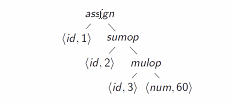
\includegraphics[width=.4\textwidth]{final-example-parsing-tree.png}
    \caption{Parsing tree ricavato dal nostro esempio}
    \label{fig:last-ex-parse-tree}
\end{figure}
Per l'analisi sintattica noi abbiamo studiato ed utilizzato le due famiglie principali di metodi di parsing (ovvero leftmost e rightmost). 
È da notare però che esistono parser adatti all'analisi di una qualsiasi grammatica libera, tuttavia questi hanno complessità minima \(n^3\) (con \(n\) lungehezza dell'input) il che li esclude dalla nostra wishlist.
I parser che abbiamo affrontato in questo testo riescono a ricavare un albero di derivazione con complessità LINEAREH.

Abbiamo visto due tipologie principali di parsing:
\begin{itemize}
    \item parsing top-down;
    \item parsing bottom-up.
\end{itemize} 

\subsection{Parsing top-down\\ \small{Quello bello}}
Quando ci troviamo al cospetto di grammatiche LL(1) riusciamo a ricavare il parse tree senza bisogno di backtrack utilizzando il parsing top-down.
La strategia di analisi del parsing top-down prevede di partire dalla derivazione dello start symbol e poi utilizzando la derivazione di tipo leftmost andare a costruire il parse tree.
Se la grammatica è LL(1) va tutto liscio ed otteniamo l'albero di parsing in men che non si dica, se non lo è dobbiamo ricorrere al backtrack, ma noi non vogliamo che questo succeda, Larry.

Abbiamo quindi visto delle caratteristiche che vogliamo evitare per assicurarci di lavorare sempre con grammatiche LL(1):
\begin{itemize}
    \item Le grammatiche ricorsive sinistre non sono LL(1), abbiamo visto però come si può, in alcuni casi, trasformarle per renderle tali;
    \item Le grammatiche fattorizzabili a sinistra non sono LL(1), ma come per il punto precedente aabbiamo visto come è possibile provare ad eliminare questo problema;
    \item Le grammatiche ambigue non sono LL(1), perché esiste almeno una stringa nel linguaggio che può essere derivata in 2 modi diversi (entrambi leftmost).
\end{itemize}

\subsection{Parsing bottom-up\\ \small{Quello tosto}}
L'altra grossa famigliola di grammatiche che abbiamo visto contiene quelle grammatiche che possono essere analizzate tramite il parsing bottom-up, di questa famiglia siamo andati ad indagare queste tipologie di grammatiche:
\begin{itemize}
    \item SLR
    \item LR(1)
    \item LALR
\end{itemize}
Il goal dell'analisi bottom-up è sempre lo stesso, ma il modo in cui si va a ricostruire l'albero di derivazione è opposto al parsing top-down: si parte a ricostruire l'albero delle derivazioni dalle foglie e si continua fino alla radice.
\\\\
Indifferentemente dal tipo di grammatica che stiamo analizzando il modo per ricavare il parse tree è sempre l'utilizzo dell'algoritmo shift-reduce.
L'algoritmo di shift-reduceè anche'esso indipendente dal tipo di grammatica che si va ad utilizzare una volta che si ottiene la parsing table per quel tipo particolare di grammatica.

Mentre eseguiamo shift reduce andiamo ad analizzare la lista di token in input token per token ed usando la parsing table come mappa ci spostiamo nel buffer di lettura (mosse di shift); quando incontriamo una stringa che può derivare da una certa produzione della grammatica andiamo ad effettuare una mossa di reduce.
Se non vi sono entry multiple defined possiamo terminare l'agloritmo con successo ed ottenere alla fine il parsing tree che tanto desideriamo.

Le 3 grammatiche che abbiamo visto per il parsing bottom-up si differenziano per quanto sono precise ed accurate le condizioni per riconoscere in quali caselle della tabella di parsing inserire una determinata mossa di riduzione.

La differenza tra un tipo di grammatica e l'altro è la seguente: utilizzando grammatiche e parsing SLR otteniamo un automa per il parsing semplice ma povero di informazioni, mentre il parsing LR(1) ci fornisce degli automi molto più precisi con dei lookahead set che ci danno molte più informazioni su quando applicare le riduzione.
Nel mezzo tra SLR e LR(1) troviamo grammatiche LALR che ci offrono una tabella di parsing delle dimensioni di una tabella SLR ma hanno una complessità di calcolo leggermente superiore alle grammatiche LR(1) e sono in grado di darci gli stessi lookahead set (quindi la stessa precisione) del parsing LR(1).

In realtà non terminano qui le possibilità, si potrebbero ottenere delle grammatiche motlo più semplici da parsare aumentantdo le informazioni che si usano prima delle riduzioni, sostanzialmente aumentando il lookahead set, tali grammatiche potrebbero essere LL(2) ed LR(2), ma la complessità per l'analisi della lista di token aumenterebbe parecchio in tal caso, quindi quello che si fa di norma è sforzarsi di trovare una grammatica LL(1) o LR(1) prima per avere performance migliori poi.

\subsection{Quando finisce il parsing}
Se l'analisi sintattica dimostra che la stringa non è riconosciuta dal linguaggio nei compilatori moderni sono previsti anche dei meccanismi di riconoscimento degli errori: spesso i compilatori stessi suggeriscono all'utente dove si prtrebbero trovare gli errori sintattici all'interno del codice.

In caso l'analisi sia andata a buon fine si ottiene un parse tree che indica quali riduzioni sono state effettuate ed in quale ordine.

\section{Analisi semantica}
Questa è la fase in cui si va a valorizzare la sequenza di token che si ricava dall'analisi lessicale; nel nostro caso quello che otterremo dall'analisi semantica ha questa forma:
\begin{figure}[H]
    \centering
    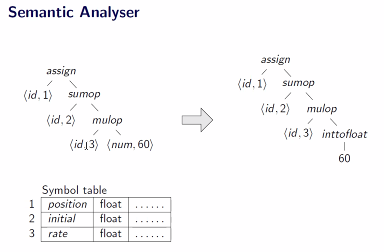
\includegraphics[width=.4\textwidth]{final-example-semantic-output.png}
    \caption{Output dell'analisi semantica}
    \label{fig:last-ex-semantic-output}
\end{figure}
Si noti che il \(<num, 60>\) è stato trasformato in \texttt{inttofloat} con nodo figlio \(60\); questo è avvenuto perchè l'analisi semantica è quella in cui si da un valore e valorizzare significa anche dare un tipo alle variabili, quindi in realtà gli effetti dell'analisi semantica non si vedranno solo nell'albero come mostrato in Fig.\ref{fig:last-ex-semantic-output} ma anche nella tabella dei simboli che riportiamo qui:
\begin{table}[H]
	\centering
	\subimport{assets/tables/}{symbol-table-updated.tex}
    \caption{Symbol table aggiornata dall'analisi semantica}
    \label{tab:last-ex-symbol-table-updated}
\end{table}
Si può immaginare, facendo qualche semplificazione, che in una parte del codice precedente a quella che stiamo analizzando noi nel nostro esempio (che ricordiamo è scritta in Eq.\ref{eq:last-ex}) avessimo dichiarato le variabili: quando l'analisi semantica raggiunge tale dichiarazione effettua una tipizzazione degli identificatori, che è appunto riportata nella tabella appena mostrata.

In seguito alla tipizzazione degli identificatori, l'analizzatore semantico vedendo che \(rate\) è di tipo float capisce che la moltiplicazione \(rate * 60\) deve essere di tipo float e va a convertire il \(60\) con l'operazione \texttt{inttofloat}.

Aggiungiamo quindi una piccola nota: la tipizzazione che viene effettuata in questa fase serve anche a calcolare gli offset necessari per la memorizzazione delle variabili che verrà effettuata al momento dell'esecuzione del programma, proprio grazie a questa manovra il compilatore riesce a descrivere che al tal programma servirà una quantità di memoria \(x\) per memorizzare una variabile di tipo \(y\).

A questo punto si passa alla generazione del codice intermedio.

\section{Generazione del codice intermedio}
Un modo molto semplice per ottenere la generazione del codice intermedio consiste nell'attraversare l'albero sintattico associando un temporaneo per ogni nodo intermedio.
Si può osservare questa strategia applicata al nostro esempio, in seguito riportiamo il codice intermedio generato partendo dal risultato datoci dall'analisi semantica (Fig.\ref{fig:last-ex-semantic-output}).
\begin{align*}
    t1 &= inttofloat(60) \\
    t2 &= id3 * t1 \\
    t3 &= id2 + t2 \\
    id1 &= t3 \\
\end{align*}
Una cosa a cui prestare attenzione è il fatto che gli identificatori \texttt{id1}, \texttt{id2} e \texttt{id3} sono riferimenti alle istanze locali degli identificatori, quindi si entra già nel territorio in cui si deve implementare un meccanismo di \emph{scope}, ma di questo parleremo in seguito.

A questo punto si passa all'ottimizzazione del codice intermedio, fase che ha le sue basi teoriche in solidissime e sofisticate prove matematiche.

\section{Ottimizzazione del codice intermedio}
Nell'esempio che stiamo trattando si riesce ad ottimizzare il codice riducendo subito il \(60\) in float ed eliminando operazioni temporanee non strettamente necessarie. Vediamo subito come risulterebbe un'ottimizzazione fatta secondo queste prerogative:
\begin{align*}
    t1 &= id3 * 60.0 \\
    id1 &= id2 + t2 \\
\end{align*}
Questa fase passa di ottimizzazione sfrutta algoriutmi su grafo facendo un'analisi di catene di definition use, cioè quand'è che una particolare entità è stata definita e, a seconda di quale sia il suo utilizzo, si può decidere ad esempio di eliminare o spostare queste dichiarazioni.

Un esempio di tali operazioni è la subexpression elimination, che prevede di sintetizzare tutte le espressioni che vengono ripetute nel codice.

Ad esempio se nel nostro codie andiamo a calcolare più volte l'eepressione \(\pi * e\) la subexpression elimination va a salvare in una variabile temporanea il risultato così da evitare di calcolarlo più e più volte sprecando risorse.

Nota che tutte queste ottimizzazioni avvengono a tempo di compliazione, nella fase statica, e sono di tipo conservativo. Questo significa che alcune occorrenze della stessa espressione possono essere eseguite in entrambi i rami di un else, quello che si fa in questo caso è assumere in modo conservativo che vengano percorsi tutti i rami di tutte le condizioni.

In sostanza le ottimizzazioni che vengono effettuate in questa fase ottimizzano ciecamente senza guardare i possibili flussi di esecuzione della logica del programma.

Nota anche che nelle fasi successive tutte le variabili dovranno essere inserite nei vari registri, qui ci saranno ulteriori ottimizzazioni, per gestire al meglio l'utilizzo dei registri, che andranno ad utilizzare algoritmi di graph coloring e altre stregonerie simili.

A valle dell'ottimizzatore del codice intermedio abbiamo il generatore del codice target.

\section{Generazione del codice target}
A questo punto possiamo finalmente tradurre il codice intermedio in codice target. Riportimo in seguito quello che otteniamo in questa fase proseguendo con il nostro esempio.
\begin{figure}[H]
    \centering
    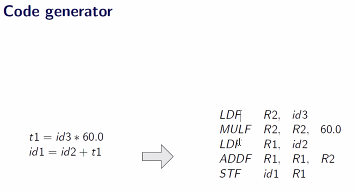
\includegraphics[width=.4\textwidth]{final-example-target-code.png}
    \caption{PHIL-PENSACI-TU}
    \label{fig:PHIL-PENSACI-TU}
\end{figure}
Spiegamo qualche dettaglio: il suffisso \texttt{F} spesso e volentieri significa float, qundi la prima riga carica il contenuto di \texttt{id3} come float in \texttt{R2}, poi avviene una moltiplicazione tra float che coinvolge \texttt{R2} e \(60\), poi un altro \texttt{load} e così via.

L'ultima nota che aggiungiamo riguardo a questa fase è che anche qui intevengono meccanismi di ottimizzazione, che però in questo caso sono strettamente legati al codice macchina.

\section{Approfondimento sulla tabella dei simboli}
Le tabelle dei simboli vengono utilizzate fin dalla fasi dell'analisi lessicale e mantenute poi per tutto il processo; si capisce bene che sono le strutture principali in un compilatore, seconde solo agli alberi di parsing.

Ma come sono implementate effettivamente? 

Ci sono varie strategie in realtà, ma la più diffusa è sicuramente la struttura dati dizionario, che deve presentare queste operazioni:
\begin{itemize}
    \item insert
    \item lookup
    \item delete
\end{itemize}
I dizionari possono essere ottenuti sia con l'utilizzo di liste che con alberi di ricerca ma l'implementazione di gran lunga più diffusa si basa sulle hash table, che offrono un costo di gestione lineare.

In questo caso si ha il canonico array bucket, dal quale si accede ad una lista di elementi che contiene tutte le entry (gli elementi della tabella dei simboli) che danno lo stesso risultato quando sono passate alla funzione di hash.

\paragraph{Funzione di hash} Com'è strutturata solitamente una funzione di hash per la tabella dei simboli di un compilatore?
Trasforma ogni carattere in un intero non negativo, tipicamente con funzioni built-in nell'implementaizone compilatore, poi su questi interi magheggia un po' per far saltare fuori l'hash.

Come si può definire una funzione di hash adeguata?
Conoscendo il dominio di applicazione. Ad esempio, nel nostro caso si può notare che spesso nella scrittura dei programmi il programmatore va a dare nomi molto similli alle variabili, quindi i caratteri iniziali degli identificatori non sono molto utili per differenziare gli identificatori stessi.

Una scelta tipicamente buona è la seguente
\begin{equation}
    (\sum_{i=1}^{n} \phi^{n-i}c_i) \; mod \; \texttt{size}
\end{equation}
Con funzioni hash di questo tipo in generale si evitano con una buona probabililtà le collisioni.

\paragraph{Scope} Ora che abbiamo discusso le metodologie di implementazione di una symbol table andiamo ad analizzare un meccanismo con cui tutte devono fare i cuonti: lo scoping.

Le dichiarazioni di fatto possono essere di due tipi: locali o globali.
Va quindi capito, se ci sono più dichiarazioni di una variabile, a quale scope si riferiscono le sue occorrenze nel codice.
Può essere utile immaginare un AST che rappresenta un certo programma in cui lo stesso nome è utilizzato sia per una variabile globale che per una variabile locale di una subroutine.
In questo ast la variabile locale sarà in un sottoalbero dell'albero in cui è dichiarata la variabile globale; le dichiarazioni locali sono comprese in sottoalberi dell'AST.

Come si va a gestire la tabella dei simboli per rispettare lo scope delle dichiarazioni?
\noindent
Esistono due principali soluzioni per gestire queste dichiarazioni annidate:
\begin{itemize}
    \item si usa un'unica symbol table e nella lista acceduta dal bucket si va a prendere la prima variabile che corrisponde a quel nome. In questo caso si è sicuri di ottenere la variabile con scope più vicino all'occorrenza che si sta analizzando perché la entry che è stata inserita per ultima sarà la prima della lista del bucket; adottando questa strategia però si deve anche implementare il meccanismo di rimozione delle variabili di uno scope quando si esce da quello scope;
    \item creiamo delle tabelle dei simboli diverse per ongi scope, in questo caso quando usciamo da uno scope ci basta cancellare il puntatore alla tabella dei simboli di quello specifico scope.
\end{itemize}

\section{Note finali per progetti futuri}
Il lettore deve sapere che esistono dei tool per la creazione di analizzatori sintattici, questi richiedono il seguente input:
\begin{itemize}
    \item una grammatica;
    \item la lista di token della grammatica; 
    \item come questi token devono interagire con l'analizzatore lessicale.
\end{itemize}
Una volta che si danno questi elementi in pasto al tool si ottiene un analizzatore sintattico bello e che funzionante. Addirittura spesso si trovano coppie di tool per la creazione di analizzatori sia lessicali che sintattici, come ad esempio la coppia di software Flex e Bison.
\\\\
Ma non è finita qui.

In alcuni casi i tool di cui sopra accettano come input anche delle funzioni di attribuzione che ci permettono di specificare le azioni semantiche per le varie produzioni (tipicamente in qualche linguaggio come il C), il che ci permette di ottenere dei parser che compiono anche la valorizzazione semantica (grazie Bison).
\\\\
Cosa significa tutto questo?

Se abbiamo un generatore di analizzatore sintattico ed un'implementazione di symbol table riusciamo a generare il nostro front-end del compilatore, poi siccome l'intermediate code può essere un qualsiasi linguaggio (spesso anche C) possiamo ottenere un compilatore in pochi semplici passi.

Alla fine quello che serve è sono solo un generatore di analizzatori sintattici, una symbol table e due pezzi di pane del giorno prima.

\end{document}
